\documentclass[1p]{elsarticle_modified}
%\bibliographystyle{elsarticle-num}

%\usepackage[colorlinks]{hyperref}
%\usepackage{abbrmath_seonhwa} %\Abb, \Ascr, \Acal ,\Abf, \Afrak
\usepackage{amsfonts}
\usepackage{amssymb}
\usepackage{amsmath}
\usepackage{amsthm}
\usepackage{scalefnt}
\usepackage{amsbsy}
\usepackage{kotex}
\usepackage{caption}
\usepackage{subfig}
\usepackage{color}
\usepackage{graphicx}
\usepackage{xcolor} %% white, black, red, green, blue, cyan, magenta, yellow
\usepackage{float}
\usepackage{setspace}
\usepackage{hyperref}

\usepackage{tikz}
\usetikzlibrary{arrows}

\usepackage{multirow}
\usepackage{array} % fixed length table
\usepackage{hhline}

%%%%%%%%%%%%%%%%%%%%%
\makeatletter
\renewcommand*\env@matrix[1][\arraystretch]{%
	\edef\arraystretch{#1}%
	\hskip -\arraycolsep
	\let\@ifnextchar\new@ifnextchar
	\array{*\c@MaxMatrixCols c}}
\makeatother %https://tex.stackexchange.com/questions/14071/how-can-i-increase-the-line-spacing-in-a-matrix
%%%%%%%%%%%%%%%

\usepackage[normalem]{ulem}

\newcommand{\msout}[1]{\ifmmode\text{\sout{\ensuremath{#1}}}\else\sout{#1}\fi}
%SOURCE: \msout is \stkout macro in https://tex.stackexchange.com/questions/20609/strikeout-in-math-mode

\newcommand{\cancel}[1]{
	\ifmmode
	{\color{red}\msout{#1}}
	\else
	{\color{red}\sout{#1}}
	\fi
}

\newcommand{\add}[1]{
	{\color{blue}\uwave{#1}}
}

\newcommand{\replace}[2]{
	\ifmmode
	{\color{red}\msout{#1}}{\color{blue}\uwave{#2}}
	\else
	{\color{red}\sout{#1}}{\color{blue}\uwave{#2}}
	\fi
}

\newcommand{\Sol}{\mathcal{S}} %segment
\newcommand{\D}{D} %diagram
\newcommand{\A}{\mathcal{A}} %arc


%%%%%%%%%%%%%%%%%%%%%%%%%%%%%5 test

\def\sl{\operatorname{\textup{SL}}(2,\Cbb)}
\def\psl{\operatorname{\textup{PSL}}(2,\Cbb)}
\def\quan{\mkern 1mu \triangleright \mkern 1mu}

\theoremstyle{definition}
\newtheorem{thm}{Theorem}[section]
\newtheorem{prop}[thm]{Proposition}
\newtheorem{lem}[thm]{Lemma}
\newtheorem{ques}[thm]{Question}
\newtheorem{cor}[thm]{Corollary}
\newtheorem{defn}[thm]{Definition}
\newtheorem{exam}[thm]{Example}
\newtheorem{rmk}[thm]{Remark}
\newtheorem{alg}[thm]{Algorithm}

\newcommand{\I}{\sqrt{-1}}
\begin{document}

%\begin{frontmatter}
%
%\title{Boundary parabolic representations of knots up to 8 crossings}
%
%%% Group authors per affiliation:
%\author{Yunhi Cho} 
%\address{Department of Mathematics, University of Seoul, Seoul, Korea}
%\ead{yhcho@uos.ac.kr}
%
%
%\author{Seonhwa Kim} %\fnref{s_kim}}
%\address{Center for Geometry and Physics, Institute for Basic Science, Pohang, 37673, Korea}
%\ead{ryeona17@ibs.re.kr}
%
%\author{Hyuk Kim}
%\address{Department of Mathematical Sciences, Seoul National University, Seoul 08826, Korea}
%\ead{hyukkim@snu.ac.kr}
%
%\author{Seokbeom Yoon}
%\address{Department of Mathematical Sciences, Seoul National University, Seoul, 08826,  Korea}
%\ead{sbyoon15@snu.ac.kr}
%
%\begin{abstract}
%We find all boundary parabolic representation of knots up to 8 crossings.
%
%\end{abstract}
%\begin{keyword}
%    \MSC[2010] 57M25 
%\end{keyword}
%
%\end{frontmatter}

%\linenumbers
%\tableofcontents
%
\newcommand\colored[1]{\textcolor{white}{\rule[-0.35ex]{0.8em}{1.4ex}}\kern-0.8em\color{red} #1}%
%\newcommand\colored[1]{\textcolor{white}{ #1}\kern-2.17ex	\textcolor{white}{ #1}\kern-1.81ex	\textcolor{white}{ #1}\kern-2.15ex\color{red}#1	}

{\Large $\underline{12n_{0151}~(K12n_{0151})}$}

\setlength{\tabcolsep}{10pt}
\renewcommand{\arraystretch}{1.6}
\vspace{1cm}\begin{tabular}{m{100pt}>{\centering\arraybackslash}m{274pt}}
\multirow{5}{120pt}{
	\centering
	\includegraphics[width=112pt]{../../../GIT/diagram.site/Diagrams/png/2240_12n_0151.png}\\
\ \ \ A knot diagram\footnotemark}&
\allowdisplaybreaks
\textbf{Linearized knot diagam} \\
\cline{2-2}
 &
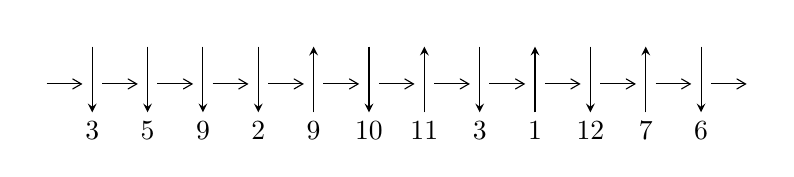
\begin{tikzpicture}[x=20pt, y=17pt]
	% nodes
	\node (C0) at (0, 0) {};
	\node (C1) at (1, 0) {};
	\node (C1U) at (1, +1) {};
	\node (C1D) at (1, -1) {3};

	\node (C2) at (2, 0) {};
	\node (C2U) at (2, +1) {};
	\node (C2D) at (2, -1) {5};

	\node (C3) at (3, 0) {};
	\node (C3U) at (3, +1) {};
	\node (C3D) at (3, -1) {9};

	\node (C4) at (4, 0) {};
	\node (C4U) at (4, +1) {};
	\node (C4D) at (4, -1) {2};

	\node (C5) at (5, 0) {};
	\node (C5U) at (5, +1) {};
	\node (C5D) at (5, -1) {9};

	\node (C6) at (6, 0) {};
	\node (C6U) at (6, +1) {};
	\node (C6D) at (6, -1) {10};

	\node (C7) at (7, 0) {};
	\node (C7U) at (7, +1) {};
	\node (C7D) at (7, -1) {11};

	\node (C8) at (8, 0) {};
	\node (C8U) at (8, +1) {};
	\node (C8D) at (8, -1) {3};

	\node (C9) at (9, 0) {};
	\node (C9U) at (9, +1) {};
	\node (C9D) at (9, -1) {1};

	\node (C10) at (10, 0) {};
	\node (C10U) at (10, +1) {};
	\node (C10D) at (10, -1) {12};

	\node (C11) at (11, 0) {};
	\node (C11U) at (11, +1) {};
	\node (C11D) at (11, -1) {7};

	\node (C12) at (12, 0) {};
	\node (C12U) at (12, +1) {};
	\node (C12D) at (12, -1) {6};
	\node (C13) at (13, 0) {};

	% arrows
	\draw[->,>={angle 60}]
	(C0) edge (C1) (C1) edge (C2) (C2) edge (C3) (C3) edge (C4) (C4) edge (C5) (C5) edge (C6) (C6) edge (C7) (C7) edge (C8) (C8) edge (C9) (C9) edge (C10) (C10) edge (C11) (C11) edge (C12) (C12) edge (C13) ;	\draw[->,>=stealth]
	(C1U) edge (C1D) (C2U) edge (C2D) (C3U) edge (C3D) (C4U) edge (C4D) (C5D) edge (C5U) (C6U) edge (C6D) (C7D) edge (C7U) (C8U) edge (C8D) (C9D) edge (C9U) (C10U) edge (C10D) (C11D) edge (C11U) (C12U) edge (C12D) ;
	\end{tikzpicture} \\
\hhline{~~} \\& 
\textbf{Solving Sequence} \\ \cline{2-2} 
 &
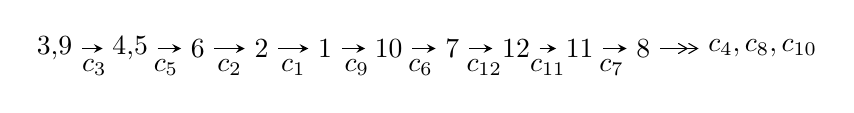
\begin{tikzpicture}[x=23pt, y=7pt]
	% node
	\node (A0) at (-1/8, 0) {3,9};
	\node (A1) at (17/16, 0) {4,5};
	\node (A2) at (17/8, 0) {6};
	\node (A3) at (25/8, 0) {2};
	\node (A4) at (33/8, 0) {1};
	\node (A5) at (41/8, 0) {10};
	\node (A6) at (49/8, 0) {7};
	\node (A7) at (57/8, 0) {12};
	\node (A8) at (65/8, 0) {11};
	\node (A9) at (73/8, 0) {8};
	\node (C1) at (1/2, -1) {$c_{3}$};
	\node (C2) at (13/8, -1) {$c_{5}$};
	\node (C3) at (21/8, -1) {$c_{2}$};
	\node (C4) at (29/8, -1) {$c_{1}$};
	\node (C5) at (37/8, -1) {$c_{9}$};
	\node (C6) at (45/8, -1) {$c_{6}$};
	\node (C7) at (53/8, -1) {$c_{12}$};
	\node (C8) at (61/8, -1) {$c_{11}$};
	\node (C9) at (69/8, -1) {$c_{7}$};
	\node (A10) at (11, 0) {$c_{4},c_{8},c_{10}$};

	% edge
	\draw[->,>=stealth]	
	(A0) edge (A1) (A1) edge (A2) (A2) edge (A3) (A3) edge (A4) (A4) edge (A5) (A5) edge (A6) (A6) edge (A7) (A7) edge (A8) (A8) edge (A9) ;
	\draw[->>,>={angle 60}]	
	(A9) edge (A10);
\end{tikzpicture} \\ 

\end{tabular} \\

\footnotetext{
The image of knot diagram is generated by the software ``\textbf{Draw programme}" developed by Andrew Bartholomew(\url{http://www.layer8.co.uk/maths/draw/index.htm\#Running-draw}), where we modified some parts for our purpose(\url{https://github.com/CATsTAILs/LinksPainter}).
}\phantom \\ \newline 
\centering \textbf{Ideals for irreducible components\footnotemark of $X_{\text{par}}$} 
 
\begin{align*}
I^u_{1}&=\langle 
3.12647\times10^{124} u^{58}+4.88388\times10^{124} u^{57}+\cdots+1.00387\times10^{125} b+4.11276\times10^{127},\\
\phantom{I^u_{1}}&\phantom{= \langle  }-3.26562\times10^{125} u^{58}-5.01296\times10^{125} u^{57}+\cdots+2.00773\times10^{125} a-4.08050\times10^{128},\\
\phantom{I^u_{1}}&\phantom{= \langle  }u^{59}+u^{58}+\cdots+2048 u+1024\rangle \\
\\
I^v_{1}&=\langle 
a,\;b-1,\;v^4+v^2- v+1\rangle \\
I^v_{2}&=\langle 
a,\;b-1,\;v^6+v^5+2 v^4+2 v^3+2 v^2+2 v+1\rangle \\
\end{align*}
\raggedright * 3 irreducible components of $\dim_{\mathbb{C}}=0$, with total 69 representations.\\
\footnotetext{All coefficients of polynomials are rational numbers. But the coefficients are sometimes approximated in decimal forms when there is not enough margin.}
\newpage
\renewcommand{\arraystretch}{1}
\centering \section*{I. $I^u_{1}= \langle 3.13\times10^{124} u^{58}+4.88\times10^{124} u^{57}+\cdots+1.00\times10^{125} b+4.11\times10^{127},\;-3.27\times10^{125} u^{58}-5.01\times10^{125} u^{57}+\cdots+2.01\times10^{125} a-4.08\times10^{128},\;u^{59}+u^{58}+\cdots+2048 u+1024 \rangle$}
\flushleft \textbf{(i) Arc colorings}\\
\begin{tabular}{m{7pt} m{180pt} m{7pt} m{180pt} }
\flushright $a_{3}=$&$\begin{pmatrix}1\\0\end{pmatrix}$ \\
\flushright $a_{9}=$&$\begin{pmatrix}0\\u\end{pmatrix}$ \\
\flushright $a_{4}=$&$\begin{pmatrix}1\\u^2\end{pmatrix}$ \\
\flushright $a_{5}=$&$\begin{pmatrix}1.62652 u^{58}+2.49682 u^{57}+\cdots+8071.87 u+2032.39\\-0.311443 u^{58}-0.486506 u^{57}+\cdots-1587.44 u-409.691\end{pmatrix}$ \\
\flushright $a_{6}=$&$\begin{pmatrix}1.62652 u^{58}+2.49682 u^{57}+\cdots+8071.87 u+2032.39\\0.364133 u^{58}+0.570656 u^{57}+\cdots+1860.49 u+481.501\end{pmatrix}$ \\
\flushright $a_{2}=$&$\begin{pmatrix}1.62652 u^{58}+2.49682 u^{57}+\cdots+8071.87 u+2032.39\\-0.364133 u^{58}-0.570656 u^{57}+\cdots-1860.49 u-481.501\end{pmatrix}$ \\
\flushright $a_{1}=$&$\begin{pmatrix}1.26239 u^{58}+1.92617 u^{57}+\cdots+6211.38 u+1550.89\\-0.364133 u^{58}-0.570656 u^{57}+\cdots-1860.49 u-481.501\end{pmatrix}$ \\
\flushright $a_{10}=$&$\begin{pmatrix}2.30700 u^{58}+0.360471 u^{57}+\cdots-4216.20 u-4797.17\\-0.565229 u^{58}-0.116297 u^{57}+\cdots+894.169 u+1106.32\end{pmatrix}$ \\
\flushright $a_{7}=$&$\begin{pmatrix}5.81545 u^{58}+7.39875 u^{57}+\cdots+21563.7 u+3635.94\\1.51836 u^{58}+2.56526 u^{57}+\cdots+8651.47 u+2450.59\end{pmatrix}$ \\
\flushright $a_{12}=$&$\begin{pmatrix}-5.75244 u^{58}-8.42872 u^{57}+\cdots-26627.9 u-6229.64\\-1.53789 u^{58}-2.31822 u^{57}+\cdots-7427.88 u-1819.55\end{pmatrix}$ \\
\flushright $a_{11}=$&$\begin{pmatrix}-4.22067 u^{58}-3.95119 u^{57}+\cdots-8869.99 u+637.146\\-2.04332 u^{58}-2.01780 u^{57}+\cdots-4729.36 u+74.4945\end{pmatrix}$ \\
\flushright $a_{8}=$&$\begin{pmatrix}- u\\- u\end{pmatrix}$\\&\end{tabular}
\flushleft \textbf{(ii) Obstruction class $= -1$}\\~\\
\flushleft \textbf{(iii) Cusp Shapes $= 12.9922 u^{58}+16.4987 u^{57}+\cdots+46831.5 u+7718.14$}\\~\\
\newpage\renewcommand{\arraystretch}{1}
\flushleft \textbf{(iv) u-Polynomials at the component}\newline \\
\begin{tabular}{m{50pt}|m{274pt}}
Crossings & \hspace{64pt}u-Polynomials at each crossing \\
\hline $$\begin{aligned}c_{1}\end{aligned}$$&$\begin{aligned}
&u^{59}+15 u^{58}+\cdots+15 u+1
\end{aligned}$\\
\hline $$\begin{aligned}c_{2},c_{4}\end{aligned}$$&$\begin{aligned}
&u^{59}-11 u^{58}+\cdots-11 u+1
\end{aligned}$\\
\hline $$\begin{aligned}c_{3},c_{8}\end{aligned}$$&$\begin{aligned}
&u^{59}+u^{58}+\cdots+2048 u+1024
\end{aligned}$\\
\hline $$\begin{aligned}c_{5}\end{aligned}$$&$\begin{aligned}
&u^{59}-2 u^{58}+\cdots+2 u+1
\end{aligned}$\\
\hline $$\begin{aligned}c_{6}\end{aligned}$$&$\begin{aligned}
&u^{59}+2 u^{58}+\cdots+480 u+72
\end{aligned}$\\
\hline $$\begin{aligned}c_{7},c_{11}\end{aligned}$$&$\begin{aligned}
&u^{59}-2 u^{58}+\cdots-4 u^2+1
\end{aligned}$\\
\hline $$\begin{aligned}c_{9}\end{aligned}$$&$\begin{aligned}
&u^{59}+8 u^{58}+\cdots+2958 u+53
\end{aligned}$\\
\hline $$\begin{aligned}c_{10}\end{aligned}$$&$\begin{aligned}
&u^{59}+28 u^{58}+\cdots+8 u-1
\end{aligned}$\\
\hline $$\begin{aligned}c_{12}\end{aligned}$$&$\begin{aligned}
&u^{59}-10 u^{58}+\cdots-1216 u+193
\end{aligned}$\\
\hline
\end{tabular}\\~\\
\newpage\renewcommand{\arraystretch}{1}
\flushleft \textbf{(v) Riley Polynomials at the component}\newline \\
\begin{tabular}{m{50pt}|m{274pt}}
Crossings & \hspace{64pt}Riley Polynomials at each crossing \\
\hline $$\begin{aligned}c_{1}\end{aligned}$$&$\begin{aligned}
&y^{59}+69 y^{58}+\cdots-13 y-1
\end{aligned}$\\
\hline $$\begin{aligned}c_{2},c_{4}\end{aligned}$$&$\begin{aligned}
&y^{59}-15 y^{58}+\cdots+15 y-1
\end{aligned}$\\
\hline $$\begin{aligned}c_{3},c_{8}\end{aligned}$$&$\begin{aligned}
&y^{59}+63 y^{58}+\cdots-22544384 y-1048576
\end{aligned}$\\
\hline $$\begin{aligned}c_{5}\end{aligned}$$&$\begin{aligned}
&y^{59}-68 y^{58}+\cdots+8 y-1
\end{aligned}$\\
\hline $$\begin{aligned}c_{6}\end{aligned}$$&$\begin{aligned}
&y^{59}-12 y^{58}+\cdots+184464 y-5184
\end{aligned}$\\
\hline $$\begin{aligned}c_{7},c_{11}\end{aligned}$$&$\begin{aligned}
&y^{59}+28 y^{58}+\cdots+8 y-1
\end{aligned}$\\
\hline $$\begin{aligned}c_{9}\end{aligned}$$&$\begin{aligned}
&y^{59}-8 y^{58}+\cdots+8867000 y-2809
\end{aligned}$\\
\hline $$\begin{aligned}c_{10}\end{aligned}$$&$\begin{aligned}
&y^{59}+8 y^{58}+\cdots+108 y-1
\end{aligned}$\\
\hline $$\begin{aligned}c_{12}\end{aligned}$$&$\begin{aligned}
&y^{59}+20 y^{58}+\cdots-93136 y-37249
\end{aligned}$\\
\hline
\end{tabular}\\~\\
\newpage\flushleft \textbf{(vi) Complex Volumes and Cusp Shapes}
$$\begin{array}{c|c|c}  
\text{Solutions to }I^u_{1}& \I (\text{vol} + \sqrt{-1}CS) & \text{Cusp shape}\\
 \hline 
\begin{aligned}
u &= -0.998103 + 0.081236 I \\
a &= \phantom{-}0.553279 + 0.202090 I \\
b &= \phantom{-}0.594657 - 0.582462 I\end{aligned}
 & -2.75669 + 1.28193 I & \phantom{-0.000000 } 0 \\ \hline\begin{aligned}
u &= -0.998103 - 0.081236 I \\
a &= \phantom{-}0.553279 - 0.202090 I \\
b &= \phantom{-}0.594657 + 0.582462 I\end{aligned}
 & -2.75669 - 1.28193 I & \phantom{-0.000000 } 0 \\ \hline\begin{aligned}
u &= \phantom{-}0.909539 + 0.365168 I \\
a &= \phantom{-}0.613308 - 0.288519 I \\
b &= \phantom{-}0.335049 + 0.628049 I\end{aligned}
 & \phantom{-}2.24694 - 1.52880 I & \phantom{-0.000000 } 0 \\ \hline\begin{aligned}
u &= \phantom{-}0.909539 - 0.365168 I \\
a &= \phantom{-}0.613308 + 0.288519 I \\
b &= \phantom{-}0.335049 - 0.628049 I\end{aligned}
 & \phantom{-}2.24694 + 1.52880 I & \phantom{-0.000000 } 0 \\ \hline\begin{aligned}
u &= -0.837696 + 0.475366 I \\
a &= \phantom{-}0.645204 + 0.335171 I \\
b &= \phantom{-}0.220526 - 0.634040 I\end{aligned}
 & \phantom{-}0.76048 - 3.15014 I & \phantom{-0.000000 } 0 \\ \hline\begin{aligned}
u &= -0.837696 - 0.475366 I \\
a &= \phantom{-}0.645204 - 0.335171 I \\
b &= \phantom{-}0.220526 + 0.634040 I\end{aligned}
 & \phantom{-}0.76048 + 3.15014 I & \phantom{-0.000000 } 0 \\ \hline\begin{aligned}
u &= \phantom{-}0.390732 + 0.845943 I \\
a &= \phantom{-}0.442369 + 0.035951 I \\
b &= \phantom{-}1.245730 - 0.182507 I\end{aligned}
 & -2.98778 + 6.48838 I & -4.00000 - 4.86755 I \\ \hline\begin{aligned}
u &= \phantom{-}0.390732 - 0.845943 I \\
a &= \phantom{-}0.442369 - 0.035951 I \\
b &= \phantom{-}1.245730 + 0.182507 I\end{aligned}
 & -2.98778 - 6.48838 I & -4.00000 + 4.86755 I \\ \hline\begin{aligned}
u &= \phantom{-}1.053350 + 0.234621 I \\
a &= \phantom{-}0.555069 - 0.252023 I \\
b &= \phantom{-}0.493660 + 0.678179 I\end{aligned}
 & \phantom{-}1.56089 - 3.52655 I & \phantom{-0.000000 } 0 \\ \hline\begin{aligned}
u &= \phantom{-}1.053350 - 0.234621 I \\
a &= \phantom{-}0.555069 + 0.252023 I \\
b &= \phantom{-}0.493660 - 0.678179 I\end{aligned}
 & \phantom{-}1.56089 + 3.52655 I & \phantom{-0.000000 } 0\\
 \hline 
 \end{array}$$\newpage$$\begin{array}{c|c|c}  
\text{Solutions to }I^u_{1}& \I (\text{vol} + \sqrt{-1}CS) & \text{Cusp shape}\\
 \hline 
\begin{aligned}
u &= \phantom{-}0.745671 + 0.508578 I \\
a &= \phantom{-}0.475006 + 0.082153 I \\
b &= \phantom{-}1.044090 - 0.353528 I\end{aligned}
 & -2.42601 - 4.17459 I & -6.95458 + 5.22656 I \\ \hline\begin{aligned}
u &= \phantom{-}0.745671 - 0.508578 I \\
a &= \phantom{-}0.475006 - 0.082153 I \\
b &= \phantom{-}1.044090 + 0.353528 I\end{aligned}
 & -2.42601 + 4.17459 I & -6.95458 - 5.22656 I \\ \hline\begin{aligned}
u &= \phantom{-}0.832959 + 0.249451 I \\
a &= \phantom{-}0.514927 + 0.109936 I \\
b &= \phantom{-}0.857363 - 0.396544 I\end{aligned}
 & -3.69687 + 2.56822 I & -10.58010 - 3.67403 I \\ \hline\begin{aligned}
u &= \phantom{-}0.832959 - 0.249451 I \\
a &= \phantom{-}0.514927 - 0.109936 I \\
b &= \phantom{-}0.857363 + 0.396544 I\end{aligned}
 & -3.69687 - 2.56822 I & -10.58010 + 3.67403 I \\ \hline\begin{aligned}
u &= -1.115200 + 0.205953 I \\
a &= \phantom{-}0.535395 + 0.248456 I \\
b &= \phantom{-}0.536821 - 0.713179 I\end{aligned}
 & -0.53472 + 8.44391 I & \phantom{-0.000000 } 0 \\ \hline\begin{aligned}
u &= -1.115200 - 0.205953 I \\
a &= \phantom{-}0.535395 - 0.248456 I \\
b &= \phantom{-}0.536821 + 0.713179 I\end{aligned}
 & -0.53472 - 8.44391 I & \phantom{-0.000000 } 0 \\ \hline\begin{aligned}
u &= -0.401206 + 0.746571 I \\
a &= \phantom{-}0.452052 - 0.037776 I \\
b &= \phantom{-}1.196800 + 0.183576 I\end{aligned}
 & -0.90878 - 1.77655 I & -1.72770 + 0.28396 I \\ \hline\begin{aligned}
u &= -0.401206 - 0.746571 I \\
a &= \phantom{-}0.452052 + 0.037776 I \\
b &= \phantom{-}1.196800 - 0.183576 I\end{aligned}
 & -0.90878 + 1.77655 I & -1.72770 - 0.28396 I \\ \hline\begin{aligned}
u &= \phantom{-}0.186981 + 0.800482 I \\
a &= \phantom{-}0.447704 + 0.017000 I \\
b &= \phantom{-}1.230400 - 0.084694 I\end{aligned}
 & -4.74840 - 0.55711 I & -7.85243 + 1.55883 I \\ \hline\begin{aligned}
u &= \phantom{-}0.186981 - 0.800482 I \\
a &= \phantom{-}0.447704 - 0.017000 I \\
b &= \phantom{-}1.230400 + 0.084694 I\end{aligned}
 & -4.74840 + 0.55711 I & -7.85243 - 1.55883 I\\
 \hline 
 \end{array}$$\newpage$$\begin{array}{c|c|c}  
\text{Solutions to }I^u_{1}& \I (\text{vol} + \sqrt{-1}CS) & \text{Cusp shape}\\
 \hline 
\begin{aligned}
u &= -0.585460 + 0.521675 I \\
a &= \phantom{-}0.476336 - 0.060057 I \\
b &= \phantom{-}1.066510 + 0.260549 I\end{aligned}
 & -0.552842 - 0.321059 I & -2.73785 - 1.45340 I \\ \hline\begin{aligned}
u &= -0.585460 - 0.521675 I \\
a &= \phantom{-}0.476336 + 0.060057 I \\
b &= \phantom{-}1.066510 - 0.260549 I\end{aligned}
 & -0.552842 + 0.321059 I & -2.73785 + 1.45340 I \\ \hline\begin{aligned}
u &= -0.344966 + 0.584974 I \\
a &= \phantom{-}0.989053 + 0.444757 I \\
b &= -0.158993 - 0.378184 I\end{aligned}
 & -0.25427 + 2.25151 I & -0.88439 - 3.01856 I \\ \hline\begin{aligned}
u &= -0.344966 - 0.584974 I \\
a &= \phantom{-}0.989053 - 0.444757 I \\
b &= -0.158993 + 0.378184 I\end{aligned}
 & -0.25427 - 2.25151 I & -0.88439 + 3.01856 I \\ \hline\begin{aligned}
u &= \phantom{-}0.005163 + 0.654757 I \\
a &= \phantom{-}2.15076 + 0.83999 I \\
b &= -0.596583 - 0.157556 I\end{aligned}
 & -3.39992 - 7.96321 I & -2.44045 + 7.77163 I \\ \hline\begin{aligned}
u &= \phantom{-}0.005163 - 0.654757 I \\
a &= \phantom{-}2.15076 - 0.83999 I \\
b &= -0.596583 + 0.157556 I\end{aligned}
 & -3.39992 + 7.96321 I & -2.44045 - 7.77163 I \\ \hline\begin{aligned}
u &= \phantom{-}0.011811 + 0.651420 I \\
a &= \phantom{-}2.00434 - 0.69962 I \\
b &= -0.555268 + 0.155236 I\end{aligned}
 & -0.95728 + 3.13895 I & \phantom{-}0.53345 - 3.94025 I \\ \hline\begin{aligned}
u &= \phantom{-}0.011811 - 0.651420 I \\
a &= \phantom{-}2.00434 + 0.69962 I \\
b &= -0.555268 - 0.155236 I\end{aligned}
 & -0.95728 - 3.13895 I & \phantom{-}0.53345 + 3.94025 I \\ \hline\begin{aligned}
u &= \phantom{-}0.111459 + 0.623363 I \\
a &= \phantom{-}1.42041 - 0.50057 I \\
b &= -0.373755 + 0.220699 I\end{aligned}
 & \phantom{-}0.62234 + 1.80022 I & \phantom{-}1.46582 - 4.56224 I \\ \hline\begin{aligned}
u &= \phantom{-}0.111459 - 0.623363 I \\
a &= \phantom{-}1.42041 + 0.50057 I \\
b &= -0.373755 - 0.220699 I\end{aligned}
 & \phantom{-}0.62234 - 1.80022 I & \phantom{-}1.46582 + 4.56224 I\\
 \hline 
 \end{array}$$\newpage$$\begin{array}{c|c|c}  
\text{Solutions to }I^u_{1}& \I (\text{vol} + \sqrt{-1}CS) & \text{Cusp shape}\\
 \hline 
\begin{aligned}
u &= -0.001805 + 0.630170 I \\
a &= \phantom{-}2.24681 + 0.44360 I \\
b &= -0.571624 - 0.084577 I\end{aligned}
 & -5.13604 - 0.16765 I & -5.11369 + 0.60296 I \\ \hline\begin{aligned}
u &= -0.001805 - 0.630170 I \\
a &= \phantom{-}2.24681 - 0.44360 I \\
b &= -0.571624 + 0.084577 I\end{aligned}
 & -5.13604 + 0.16765 I & -5.11369 - 0.60296 I \\ \hline\begin{aligned}
u &= -0.579721\phantom{ +0.000000I} \\
a &= \phantom{-}0.575386\phantom{ +0.000000I} \\
b &= \phantom{-}0.737962\phantom{ +0.000000I}\end{aligned}
 & -1.10396\phantom{ +0.000000I} & -8.80140\phantom{ +0.000000I} \\ \hline\begin{aligned}
u &= \phantom{-}0.19820 + 1.41485 I \\
a &= \phantom{-}0.168080 + 1.201160 I \\
b &= -0.885740 - 0.816541 I\end{aligned}
 & \phantom{-}0.693286 + 0.866196 I & \phantom{-0.000000 } 0 \\ \hline\begin{aligned}
u &= \phantom{-}0.19820 - 1.41485 I \\
a &= \phantom{-}0.168080 - 1.201160 I \\
b &= -0.885740 + 0.816541 I\end{aligned}
 & \phantom{-}0.693286 - 0.866196 I & \phantom{-0.000000 } 0 \\ \hline\begin{aligned}
u &= \phantom{-}0.33794 + 1.44689 I \\
a &= \phantom{-}0.034774 + 1.229800 I \\
b &= -0.977026 - 0.812488 I\end{aligned}
 & \phantom{-}0.40044 - 7.01056 I & \phantom{-0.000000 } 0 \\ \hline\begin{aligned}
u &= \phantom{-}0.33794 - 1.44689 I \\
a &= \phantom{-}0.034774 - 1.229800 I \\
b &= -0.977026 + 0.812488 I\end{aligned}
 & \phantom{-}0.40044 + 7.01056 I & \phantom{-0.000000 } 0 \\ \hline\begin{aligned}
u &= -0.25718 + 1.49968 I \\
a &= \phantom{-}0.084876 - 1.159550 I \\
b &= -0.937211 + 0.857810 I\end{aligned}
 & \phantom{-}3.75772 + 3.20443 I & \phantom{-0.000000 } 0 \\ \hline\begin{aligned}
u &= -0.25718 - 1.49968 I \\
a &= \phantom{-}0.084876 + 1.159550 I \\
b &= -0.937211 - 0.857810 I\end{aligned}
 & \phantom{-}3.75772 - 3.20443 I & \phantom{-0.000000 } 0 \\ \hline\begin{aligned}
u &= \phantom{-}0.04696 + 1.65800 I \\
a &= \phantom{-}0.193873 - 0.944416 I \\
b &= -0.791424 + 1.016040 I\end{aligned}
 & \phantom{-}3.69904 - 0.23163 I & \phantom{-0.000000 } 0\\
 \hline 
 \end{array}$$\newpage$$\begin{array}{c|c|c}  
\text{Solutions to }I^u_{1}& \I (\text{vol} + \sqrt{-1}CS) & \text{Cusp shape}\\
 \hline 
\begin{aligned}
u &= \phantom{-}0.04696 - 1.65800 I \\
a &= \phantom{-}0.193873 + 0.944416 I \\
b &= -0.791424 - 1.016040 I\end{aligned}
 & \phantom{-}3.69904 + 0.23163 I & \phantom{-0.000000 } 0 \\ \hline\begin{aligned}
u &= -0.50336 + 1.59145 I \\
a &= -0.123627 - 1.133430 I \\
b &= -1.095100 + 0.871905 I\end{aligned}
 & \phantom{-}2.73059 + 7.14739 I & \phantom{-0.000000 } 0 \\ \hline\begin{aligned}
u &= -0.50336 - 1.59145 I \\
a &= -0.123627 + 1.133430 I \\
b &= -1.095100 - 0.871905 I\end{aligned}
 & \phantom{-}2.73059 - 7.14739 I & \phantom{-0.000000 } 0 \\ \hline\begin{aligned}
u &= \phantom{-}0.53071 + 1.64437 I \\
a &= -0.144074 + 1.095240 I \\
b &= -1.11806 - 0.89751 I\end{aligned}
 & \phantom{-}7.55867 - 9.77831 I & \phantom{-0.000000 } 0 \\ \hline\begin{aligned}
u &= \phantom{-}0.53071 - 1.64437 I \\
a &= -0.144074 - 1.095240 I \\
b &= -1.11806 + 0.89751 I\end{aligned}
 & \phantom{-}7.55867 + 9.77831 I & \phantom{-0.000000 } 0 \\ \hline\begin{aligned}
u &= -0.55751 + 1.63560 I \\
a &= -0.163068 - 1.100950 I \\
b &= -1.13165 + 0.88881 I\end{aligned}
 & \phantom{-}5.3016 + 14.9246 I & \phantom{-0.000000 } 0 \\ \hline\begin{aligned}
u &= -0.55751 - 1.63560 I \\
a &= -0.163068 + 1.100950 I \\
b &= -1.13165 - 0.88881 I\end{aligned}
 & \phantom{-}5.3016 - 14.9246 I & \phantom{-0.000000 } 0 \\ \hline\begin{aligned}
u &= \phantom{-}0.45548 + 1.68569 I \\
a &= -0.094411 + 1.064750 I \\
b &= -1.08263 - 0.93187 I\end{aligned}
 & \phantom{-}8.89235 - 7.23820 I & \phantom{-0.000000 } 0 \\ \hline\begin{aligned}
u &= \phantom{-}0.45548 - 1.68569 I \\
a &= -0.094411 - 1.064750 I \\
b &= -1.08263 + 0.93187 I\end{aligned}
 & \phantom{-}8.89235 + 7.23820 I & \phantom{-0.000000 } 0 \\ \hline\begin{aligned}
u &= -0.06440 + 1.74963 I \\
a &= \phantom{-}0.164970 + 0.902532 I \\
b &= -0.804022 - 1.072170 I\end{aligned}
 & \phantom{-}8.58017 + 2.61249 I & \phantom{-0.000000 } 0\\
 \hline 
 \end{array}$$\newpage$$\begin{array}{c|c|c}  
\text{Solutions to }I^u_{1}& \I (\text{vol} + \sqrt{-1}CS) & \text{Cusp shape}\\
 \hline 
\begin{aligned}
u &= -0.06440 - 1.74963 I \\
a &= \phantom{-}0.164970 - 0.902532 I \\
b &= -0.804022 + 1.072170 I\end{aligned}
 & \phantom{-}8.58017 - 2.61249 I & \phantom{-0.000000 } 0 \\ \hline\begin{aligned}
u &= -0.40556 + 1.70511 I \\
a &= -0.064015 - 1.047870 I \\
b &= -1.05808 + 0.95077 I\end{aligned}
 & \phantom{-}7.86608 + 2.22410 I & \phantom{-0.000000 } 0 \\ \hline\begin{aligned}
u &= -0.40556 - 1.70511 I \\
a &= -0.064015 + 1.047870 I \\
b &= -1.05808 - 0.95077 I\end{aligned}
 & \phantom{-}7.86608 - 2.22410 I & \phantom{-0.000000 } 0 \\ \hline\begin{aligned}
u &= \phantom{-}0.10531 + 1.75148 I \\
a &= \phantom{-}0.178722 - 0.887018 I \\
b &= -0.781712 + 1.083390 I\end{aligned}
 & \phantom{-}6.43786 - 7.75949 I & \phantom{-0.000000 } 0 \\ \hline\begin{aligned}
u &= \phantom{-}0.10531 - 1.75148 I \\
a &= \phantom{-}0.178722 + 0.887018 I \\
b &= -0.781712 - 1.083390 I\end{aligned}
 & \phantom{-}6.43786 + 7.75949 I & \phantom{-0.000000 } 0 \\ \hline\begin{aligned}
u &= \phantom{-}0.04475 + 1.76538 I \\
a &= \phantom{-}0.116249 + 0.933213 I \\
b &= -0.868556 - 1.055190 I\end{aligned}
 & \phantom{-}9.59397 + 0.00079 I & \phantom{-0.000000 } 0 \\ \hline\begin{aligned}
u &= \phantom{-}0.04475 - 1.76538 I \\
a &= \phantom{-}0.116249 - 0.933213 I \\
b &= -0.868556 + 1.055190 I\end{aligned}
 & \phantom{-}9.59397 - 0.00079 I & \phantom{-0.000000 } 0 \\ \hline\begin{aligned}
u &= -0.10471 + 1.77099 I \\
a &= \phantom{-}0.087935 - 0.948757 I \\
b &= -0.903142 + 1.045030 I\end{aligned}
 & \phantom{-}8.37962 + 5.04404 I & \phantom{-0.000000 } 0 \\ \hline\begin{aligned}
u &= -0.10471 - 1.77099 I \\
a &= \phantom{-}0.087935 + 0.948757 I \\
b &= -0.903142 - 1.045030 I\end{aligned}
 & \phantom{-}8.37962 - 5.04404 I & \phantom{-0.000000 } 0\\
 \hline 
 \end{array}$$\newpage\newpage\renewcommand{\arraystretch}{1}
\centering \section*{II. $I^v_{1}= \langle a,\;b-1,\;v^4+v^2- v+1 \rangle$}
\flushleft \textbf{(i) Arc colorings}\\
\begin{tabular}{m{7pt} m{180pt} m{7pt} m{180pt} }
\flushright $a_{3}=$&$\begin{pmatrix}1\\0\end{pmatrix}$ \\
\flushright $a_{9}=$&$\begin{pmatrix}v\\0\end{pmatrix}$ \\
\flushright $a_{4}=$&$\begin{pmatrix}1\\0\end{pmatrix}$ \\
\flushright $a_{5}=$&$\begin{pmatrix}0\\1\end{pmatrix}$ \\
\flushright $a_{6}=$&$\begin{pmatrix}v^2\\1\end{pmatrix}$ \\
\flushright $a_{2}=$&$\begin{pmatrix}1\\-1\end{pmatrix}$ \\
\flushright $a_{1}=$&$\begin{pmatrix}0\\-1\end{pmatrix}$ \\
\flushright $a_{10}=$&$\begin{pmatrix}v\\- v\end{pmatrix}$ \\
\flushright $a_{7}=$&$\begin{pmatrix}v^2- v+1\\v\end{pmatrix}$ \\
\flushright $a_{12}=$&$\begin{pmatrix}v^2- v+1\\- v^2-1\end{pmatrix}$ \\
\flushright $a_{11}=$&$\begin{pmatrix}v^3+1\\-1\end{pmatrix}$ \\
\flushright $a_{8}=$&$\begin{pmatrix}v\\0\end{pmatrix}$\\&\end{tabular}
\flushleft \textbf{(ii) Obstruction class $= 1$}\\~\\
\flushleft \textbf{(iii) Cusp Shapes $= -5 v^3-4 v^2- v-6$}\\~\\
\newpage\renewcommand{\arraystretch}{1}
\flushleft \textbf{(iv) u-Polynomials at the component}\newline \\
\begin{tabular}{m{50pt}|m{274pt}}
Crossings & \hspace{64pt}u-Polynomials at each crossing \\
\hline $$\begin{aligned}c_{1},c_{2}\end{aligned}$$&$\begin{aligned}
&(u-1)^4
\end{aligned}$\\
\hline $$\begin{aligned}c_{3},c_{8}\end{aligned}$$&$\begin{aligned}
&u^4
\end{aligned}$\\
\hline $$\begin{aligned}c_{4}\end{aligned}$$&$\begin{aligned}
&(u+1)^4
\end{aligned}$\\
\hline $$\begin{aligned}c_{5},c_{7},c_{9}\end{aligned}$$&$\begin{aligned}
&u^4+u^2+u+1
\end{aligned}$\\
\hline $$\begin{aligned}c_{6}\end{aligned}$$&$\begin{aligned}
&u^4+3 u^3+4 u^2+3 u+2
\end{aligned}$\\
\hline $$\begin{aligned}c_{10}\end{aligned}$$&$\begin{aligned}
&u^4-2 u^3+3 u^2- u+1
\end{aligned}$\\
\hline $$\begin{aligned}c_{11}\end{aligned}$$&$\begin{aligned}
&u^4+u^2- u+1
\end{aligned}$\\
\hline $$\begin{aligned}c_{12}\end{aligned}$$&$\begin{aligned}
&u^4+2 u^3+3 u^2+u+1
\end{aligned}$\\
\hline
\end{tabular}\\~\\
\newpage\renewcommand{\arraystretch}{1}
\flushleft \textbf{(v) Riley Polynomials at the component}\newline \\
\begin{tabular}{m{50pt}|m{274pt}}
Crossings & \hspace{64pt}Riley Polynomials at each crossing \\
\hline $$\begin{aligned}c_{1},c_{2},c_{4}\end{aligned}$$&$\begin{aligned}
&(y-1)^4
\end{aligned}$\\
\hline $$\begin{aligned}c_{3},c_{8}\end{aligned}$$&$\begin{aligned}
&y^4
\end{aligned}$\\
\hline $$\begin{aligned}c_{5},c_{7},c_{9}\\c_{11}\end{aligned}$$&$\begin{aligned}
&y^4+2 y^3+3 y^2+y+1
\end{aligned}$\\
\hline $$\begin{aligned}c_{6}\end{aligned}$$&$\begin{aligned}
&y^4- y^3+2 y^2+7 y+4
\end{aligned}$\\
\hline $$\begin{aligned}c_{10},c_{12}\end{aligned}$$&$\begin{aligned}
&y^4+2 y^3+7 y^2+5 y+1
\end{aligned}$\\
\hline
\end{tabular}\\~\\
\newpage\flushleft \textbf{(vi) Complex Volumes and Cusp Shapes}
$$\begin{array}{c|c|c}  
\text{Solutions to }I^v_{1}& \I (\text{vol} + \sqrt{-1}CS) & \text{Cusp shape}\\
 \hline 
\begin{aligned}
v &= \phantom{-}0.547424 + 0.585652 I \\
a &= \phantom{-0.000000 } 0 \\
b &= \phantom{-}1.00000\phantom{ +0.000000I}\end{aligned}
 & -0.66484 + 1.39709 I & -4.37800 - 4.77865 I \\ \hline\begin{aligned}
v &= \phantom{-}0.547424 - 0.585652 I \\
a &= \phantom{-0.000000 } 0 \\
b &= \phantom{-}1.00000\phantom{ +0.000000I}\end{aligned}
 & -0.66484 - 1.39709 I & -4.37800 + 4.77865 I \\ \hline\begin{aligned}
v &= -0.547424 + 1.120870 I \\
a &= \phantom{-0.000000 } 0 \\
b &= \phantom{-}1.00000\phantom{ +0.000000I}\end{aligned}
 & -4.26996 - 7.64338 I & -11.12200 + 5.79053 I \\ \hline\begin{aligned}
v &= -0.547424 - 1.120870 I \\
a &= \phantom{-0.000000 } 0 \\
b &= \phantom{-}1.00000\phantom{ +0.000000I}\end{aligned}
 & -4.26996 + 7.64338 I & -11.12200 - 5.79053 I\\
 \hline 
 \end{array}$$\newpage\newpage\renewcommand{\arraystretch}{1}
\centering \section*{III. $I^v_{2}= \langle a,\;b-1,\;v^6+v^5+2 v^4+2 v^3+2 v^2+2 v+1 \rangle$}
\flushleft \textbf{(i) Arc colorings}\\
\begin{tabular}{m{7pt} m{180pt} m{7pt} m{180pt} }
\flushright $a_{3}=$&$\begin{pmatrix}1\\0\end{pmatrix}$ \\
\flushright $a_{9}=$&$\begin{pmatrix}v\\0\end{pmatrix}$ \\
\flushright $a_{4}=$&$\begin{pmatrix}1\\0\end{pmatrix}$ \\
\flushright $a_{5}=$&$\begin{pmatrix}0\\1\end{pmatrix}$ \\
\flushright $a_{6}=$&$\begin{pmatrix}v^2\\1\end{pmatrix}$ \\
\flushright $a_{2}=$&$\begin{pmatrix}1\\-1\end{pmatrix}$ \\
\flushright $a_{1}=$&$\begin{pmatrix}0\\-1\end{pmatrix}$ \\
\flushright $a_{10}=$&$\begin{pmatrix}v\\- v\end{pmatrix}$ \\
\flushright $a_{7}=$&$\begin{pmatrix}- v^4\\v^4+v^2+1\end{pmatrix}$ \\
\flushright $a_{12}=$&$\begin{pmatrix}- v^4\\- v^2-1\end{pmatrix}$ \\
\flushright $a_{11}=$&$\begin{pmatrix}v^5+v^3+v^2+v\\v^5+2 v^3+v+1\end{pmatrix}$ \\
\flushright $a_{8}=$&$\begin{pmatrix}v\\0\end{pmatrix}$\\&\end{tabular}
\flushleft \textbf{(ii) Obstruction class $= 1$}\\~\\
\flushleft \textbf{(iii) Cusp Shapes $= 2 v^5+v^4- v^3+3 v^2-2 v-8$}\\~\\
\newpage\renewcommand{\arraystretch}{1}
\flushleft \textbf{(iv) u-Polynomials at the component}\newline \\
\begin{tabular}{m{50pt}|m{274pt}}
Crossings & \hspace{64pt}u-Polynomials at each crossing \\
\hline $$\begin{aligned}c_{1},c_{2}\end{aligned}$$&$\begin{aligned}
&(u-1)^6
\end{aligned}$\\
\hline $$\begin{aligned}c_{3},c_{8}\end{aligned}$$&$\begin{aligned}
&u^6
\end{aligned}$\\
\hline $$\begin{aligned}c_{4}\end{aligned}$$&$\begin{aligned}
&(u+1)^6
\end{aligned}$\\
\hline $$\begin{aligned}c_{5},c_{7},c_{9}\end{aligned}$$&$\begin{aligned}
&u^6- u^5+2 u^4-2 u^3+2 u^2-2 u+1
\end{aligned}$\\
\hline $$\begin{aligned}c_{6}\end{aligned}$$&$\begin{aligned}
&(u^3- u^2+1)^2
\end{aligned}$\\
\hline $$\begin{aligned}c_{10}\end{aligned}$$&$\begin{aligned}
&u^6-3 u^5+4 u^4-2 u^3+1
\end{aligned}$\\
\hline $$\begin{aligned}c_{11}\end{aligned}$$&$\begin{aligned}
&u^6+u^5+2 u^4+2 u^3+2 u^2+2 u+1
\end{aligned}$\\
\hline $$\begin{aligned}c_{12}\end{aligned}$$&$\begin{aligned}
&u^6+3 u^5+4 u^4+2 u^3+1
\end{aligned}$\\
\hline
\end{tabular}\\~\\
\newpage\renewcommand{\arraystretch}{1}
\flushleft \textbf{(v) Riley Polynomials at the component}\newline \\
\begin{tabular}{m{50pt}|m{274pt}}
Crossings & \hspace{64pt}Riley Polynomials at each crossing \\
\hline $$\begin{aligned}c_{1},c_{2},c_{4}\end{aligned}$$&$\begin{aligned}
&(y-1)^6
\end{aligned}$\\
\hline $$\begin{aligned}c_{3},c_{8}\end{aligned}$$&$\begin{aligned}
&y^6
\end{aligned}$\\
\hline $$\begin{aligned}c_{5},c_{7},c_{9}\\c_{11}\end{aligned}$$&$\begin{aligned}
&y^6+3 y^5+4 y^4+2 y^3+1
\end{aligned}$\\
\hline $$\begin{aligned}c_{6}\end{aligned}$$&$\begin{aligned}
&(y^3- y^2+2 y-1)^2
\end{aligned}$\\
\hline $$\begin{aligned}c_{10},c_{12}\end{aligned}$$&$\begin{aligned}
&y^6- y^5+4 y^4-2 y^3+8 y^2+1
\end{aligned}$\\
\hline
\end{tabular}\\~\\
\newpage\flushleft \textbf{(vi) Complex Volumes and Cusp Shapes}
$$\begin{array}{c|c|c}  
\text{Solutions to }I^v_{2}& \I (\text{vol} + \sqrt{-1}CS) & \text{Cusp shape}\\
 \hline 
\begin{aligned}
v &= \phantom{-}0.498832 + 1.001300 I \\
a &= \phantom{-0.000000 } 0 \\
b &= \phantom{-}1.00000\phantom{ +0.000000I}\end{aligned}
 & -1.91067 + 2.82812 I & -7.72532 - 2.61835 I \\ \hline\begin{aligned}
v &= \phantom{-}0.498832 - 1.001300 I \\
a &= \phantom{-0.000000 } 0 \\
b &= \phantom{-}1.00000\phantom{ +0.000000I}\end{aligned}
 & -1.91067 - 2.82812 I & -7.72532 + 2.61835 I \\ \hline\begin{aligned}
v &= -0.284920 + 1.115140 I \\
a &= \phantom{-0.000000 } 0 \\
b &= \phantom{-}1.00000\phantom{ +0.000000I}\end{aligned}
 & -6.04826\phantom{ +0.000000I} & -14.8442 - 0.2733 I \\ \hline\begin{aligned}
v &= -0.284920 - 1.115140 I \\
a &= \phantom{-0.000000 } 0 \\
b &= \phantom{-}1.00000\phantom{ +0.000000I}\end{aligned}
 & -6.04826\phantom{ +0.000000I} & -14.8442 + 0.2733 I \\ \hline\begin{aligned}
v &= -0.713912 + 0.305839 I \\
a &= \phantom{-0.000000 } 0 \\
b &= \phantom{-}1.00000\phantom{ +0.000000I}\end{aligned}
 & -1.91067 + 2.82812 I & -4.93045 - 2.21599 I \\ \hline\begin{aligned}
v &= -0.713912 - 0.305839 I \\
a &= \phantom{-0.000000 } 0 \\
b &= \phantom{-}1.00000\phantom{ +0.000000I}\end{aligned}
 & -1.91067 - 2.82812 I & -4.93045 + 2.21599 I\\
 \hline 
 \end{array}$$\newpage
\newpage\renewcommand{\arraystretch}{1}
\centering \section*{ IV. u-Polynomials}
\begin{tabular}{m{50pt}|m{274pt}}
Crossings & \hspace{64pt}u-Polynomials at each crossing \\
\hline $$\begin{aligned}c_{1}\end{aligned}$$&$\begin{aligned}
&((u-1)^{10})(u^{59}+15 u^{58}+\cdots+15 u+1)
\end{aligned}$\\
\hline $$\begin{aligned}c_{2}\end{aligned}$$&$\begin{aligned}
&((u-1)^{10})(u^{59}-11 u^{58}+\cdots-11 u+1)
\end{aligned}$\\
\hline $$\begin{aligned}c_{3},c_{8}\end{aligned}$$&$\begin{aligned}
&u^{10}(u^{59}+u^{58}+\cdots+2048 u+1024)
\end{aligned}$\\
\hline $$\begin{aligned}c_{4}\end{aligned}$$&$\begin{aligned}
&((u+1)^{10})(u^{59}-11 u^{58}+\cdots-11 u+1)
\end{aligned}$\\
\hline $$\begin{aligned}c_{5}\end{aligned}$$&$\begin{aligned}
&(u^4+u^2+u+1)(u^6- u^5+2 u^4-2 u^3+2 u^2-2 u+1)\\
&\cdot(u^{59}-2 u^{58}+\cdots+2 u+1)
\end{aligned}$\\
\hline $$\begin{aligned}c_{6}\end{aligned}$$&$\begin{aligned}
&((u^3- u^2+1)^2)(u^4+3 u^3+\cdots+3 u+2)(u^{59}+2 u^{58}+\cdots+480 u+72)
\end{aligned}$\\
\hline $$\begin{aligned}c_{7}\end{aligned}$$&$\begin{aligned}
&(u^4+u^2+u+1)(u^6- u^5+2 u^4-2 u^3+2 u^2-2 u+1)\\
&\cdot(u^{59}-2 u^{58}+\cdots-4 u^2+1)
\end{aligned}$\\
\hline $$\begin{aligned}c_{9}\end{aligned}$$&$\begin{aligned}
&(u^4+u^2+u+1)(u^6- u^5+2 u^4-2 u^3+2 u^2-2 u+1)\\
&\cdot(u^{59}+8 u^{58}+\cdots+2958 u+53)
\end{aligned}$\\
\hline $$\begin{aligned}c_{10}\end{aligned}$$&$\begin{aligned}
&(u^4-2 u^3+3 u^2- u+1)(u^6-3 u^5+4 u^4-2 u^3+1)\\
&\cdot(u^{59}+28 u^{58}+\cdots+8 u-1)
\end{aligned}$\\
\hline $$\begin{aligned}c_{11}\end{aligned}$$&$\begin{aligned}
&(u^4+u^2- u+1)(u^6+u^5+2 u^4+2 u^3+2 u^2+2 u+1)\\
&\cdot(u^{59}-2 u^{58}+\cdots-4 u^2+1)
\end{aligned}$\\
\hline $$\begin{aligned}c_{12}\end{aligned}$$&$\begin{aligned}
&(u^4+2 u^3+3 u^2+u+1)(u^6+3 u^5+4 u^4+2 u^3+1)\\
&\cdot(u^{59}-10 u^{58}+\cdots-1216 u+193)
\end{aligned}$\\
\hline
\end{tabular}\newpage\renewcommand{\arraystretch}{1}
\centering \section*{ V. Riley Polynomials}
\begin{tabular}{m{50pt}|m{274pt}}
Crossings & \hspace{64pt}Riley Polynomials at each crossing \\
\hline $$\begin{aligned}c_{1}\end{aligned}$$&$\begin{aligned}
&((y-1)^{10})(y^{59}+69 y^{58}+\cdots-13 y-1)
\end{aligned}$\\
\hline $$\begin{aligned}c_{2},c_{4}\end{aligned}$$&$\begin{aligned}
&((y-1)^{10})(y^{59}-15 y^{58}+\cdots+15 y-1)
\end{aligned}$\\
\hline $$\begin{aligned}c_{3},c_{8}\end{aligned}$$&$\begin{aligned}
&y^{10}(y^{59}+63 y^{58}+\cdots-2.25444\times10^{7} y-1048576)
\end{aligned}$\\
\hline $$\begin{aligned}c_{5}\end{aligned}$$&$\begin{aligned}
&(y^4+2 y^3+3 y^2+y+1)(y^6+3 y^5+4 y^4+2 y^3+1)\\
&\cdot(y^{59}-68 y^{58}+\cdots+8 y-1)
\end{aligned}$\\
\hline $$\begin{aligned}c_{6}\end{aligned}$$&$\begin{aligned}
&(y^3- y^2+2 y-1)^2(y^4- y^3+2 y^2+7 y+4)\\
&\cdot(y^{59}-12 y^{58}+\cdots+184464 y-5184)
\end{aligned}$\\
\hline $$\begin{aligned}c_{7},c_{11}\end{aligned}$$&$\begin{aligned}
&(y^4+2 y^3+3 y^2+y+1)(y^6+3 y^5+4 y^4+2 y^3+1)\\
&\cdot(y^{59}+28 y^{58}+\cdots+8 y-1)
\end{aligned}$\\
\hline $$\begin{aligned}c_{9}\end{aligned}$$&$\begin{aligned}
&(y^4+2 y^3+3 y^2+y+1)(y^6+3 y^5+4 y^4+2 y^3+1)\\
&\cdot(y^{59}-8 y^{58}+\cdots+8867000 y-2809)
\end{aligned}$\\
\hline $$\begin{aligned}c_{10}\end{aligned}$$&$\begin{aligned}
&(y^4+2 y^3+7 y^2+5 y+1)(y^6- y^5+4 y^4-2 y^3+8 y^2+1)\\
&\cdot(y^{59}+8 y^{58}+\cdots+108 y-1)
\end{aligned}$\\
\hline $$\begin{aligned}c_{12}\end{aligned}$$&$\begin{aligned}
&(y^4+2 y^3+7 y^2+5 y+1)(y^6- y^5+4 y^4-2 y^3+8 y^2+1)\\
&\cdot(y^{59}+20 y^{58}+\cdots-93136 y-37249)
\end{aligned}$\\
\hline
\end{tabular}
\vskip 2pc
\end{document}